\section{Auswertung}
\label{sec:Auswertung}

Für die Auswertung wird Python und im Speziellen Matplotlib \cite{matplotlib}, SciPy \cite{scipy}, Uncertainties \cite{uncertainties} und NumPy \cite{numpy} verwendet.

\subsection{Bestimmung des Energieverlustes von Alphastrahlung in Luft}

\subsubsection{Erster Abstand}
Die Drücke, die Anzahl der Pulse und die Position des jeweiligen Maximums für den Abstand $d_1 = \SI{2.7}{\centi\meter}$ in Tab. \ref{taba} zu sehen.
 
 \begin{table}\caption{Die Länge der Zylinder und die Spannung mit den jeweiligen Zeitenpunkten der Ausschläge.}
\label{taba}
\centering
\sisetup{round-mode = places, round-precision=2, round-integer-to-decimal=true}
\begin{tabular}{S[]S[]S[]S[]S[]} 
\toprule
{$l/ \si{\milli\meter}$} & {$U_1/ \si{\volt}$} & {$t_1/ \si{\micro\second}$} & {$U_2/ \si{\volt}$} & {$t_2/ \si{\micro\second}$}\\
\midrule
120.8 & 1.29 & 0.6 & 0.17 & 88.7\\
102.3 & 1.27 & 0.5 & 0.2 & 76.5\\
80.5 & 1.33 & 0.6 & 0.76 & 59.8\\
40.4 & 1.33 & 0.5 & 1.34 & 30.2\\
31.1 & 1.29 & 0.5 & 1.37 & 23.8\\
\bottomrule
\end{tabular}\end{table}

%Zählrate als Funktion der effektiven Länge für den ersten Abstand
\noindent Die mit Gleichung \eqref{eqn:x} ermittelten Abstände, die Anzahl der Pulse (Zählrate) und die mit Gleichung \eqref{eqn:energie} ermittelten Energien befinden sich in Tab. \ref{tab1}. 

 \begin{table}\caption{Der maximale Drehimpuls $L$, der Gesamtspin $S$ und der Gesamtdrehimpuls $J$ ergeben sich zum Landé-Faktor $g_\text{J}$ für die vier verschiedenen Elemente.}
\label{tab1}
\centering
\sisetup{round-mode = places, round-precision=2, round-integer-to-decimal=true}
\begin{tabular}{S[]S[]S[]S[]} 
\toprule
{$L$} & {$S$} & {$J$} & {$g_\text{J}$}\\
\midrule
5.0 & 1.0 & 4.0 & 0.8\\
0.0 & 3.5 & 3.5 & 2.0\\
6.0 & 1.5 & 4.5 & 0.7272727272727273\\
5.0 & 2.5 & 7.5 & 1.3333333333333333\\
\bottomrule
\end{tabular}\end{table}

\noindent Die Zählrate ist in Abb. \ref{zaehlrate1} gegen die mit Gleichung \eqref{eqn:x} bestimmte effektive Länge aufgetragen.

\begin{figure}
    \centering
    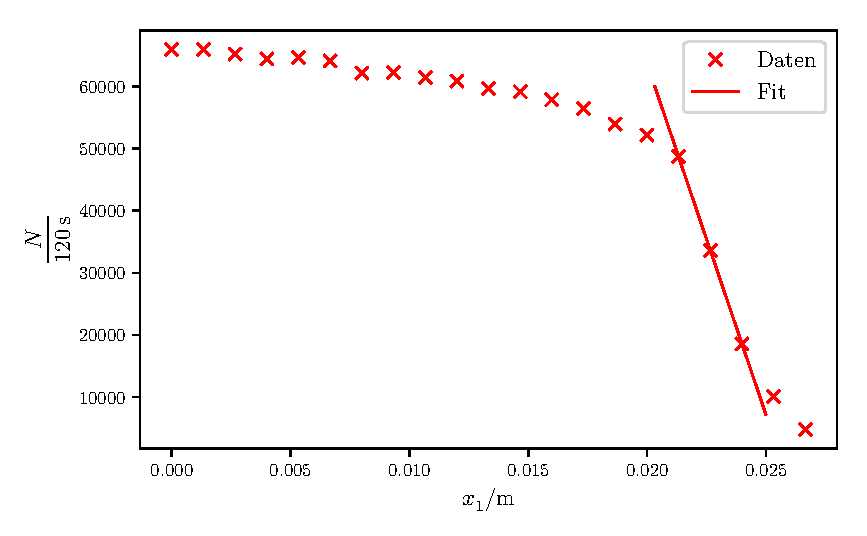
\includegraphics[width=15cm, height=9cm]{build/plota.pdf}
    \caption{Anzahl der Hits pro zwei Minuten Messzeit ist hier gegen den Abstand aufgetragen. Dabei wurde dieses Ergebnis durch die Abhängigkeit vom jeweiligen Druck ermittelt.}
    \label{zaehlrate1}
\end{figure}

\noindent Die Fitparameter der linearen Regression ergeben sich dadurch zu 
\begin{align*}
    m &= - \num{11300.95(325)} \,\frac{\text{N}}{\SI{120}{\second}\, \si{\milli\meter}} \\
    n &= \num{289663.5} \, \frac{\text{N}}{\SI{120}{\second}} .
\end{align*}


\noindent Mit dem Umformen dieser linearen Gleichung ergibt sich bei $y = \frac{1}{2} N_{max}$ die mittlere Reichweite der $\alpha$-Teilchen zu dem Wert %wie genau?
\begin{equation*}
    R_\text{m,1} = \SI{22.71(1)}{\milli\meter}
\end{equation*}
bestimmen.

\noindent Das entspricht nach Formel \eqref{eqn:Rm} einer Energie von %wie genau?
\begin{equation*}
    E_1 = \SI{3.772(1)}{\mega\electronvolt}.
\end{equation*}

%Energie als Funktion der effektiven Länge für den ersten Abstand
\noindent Die Energie aus Tab. \ref{tab1} ist in Abb. \ref{fig:energie1} gegen die effektive Länge aufgetragen.
\begin{figure}
    \centering
    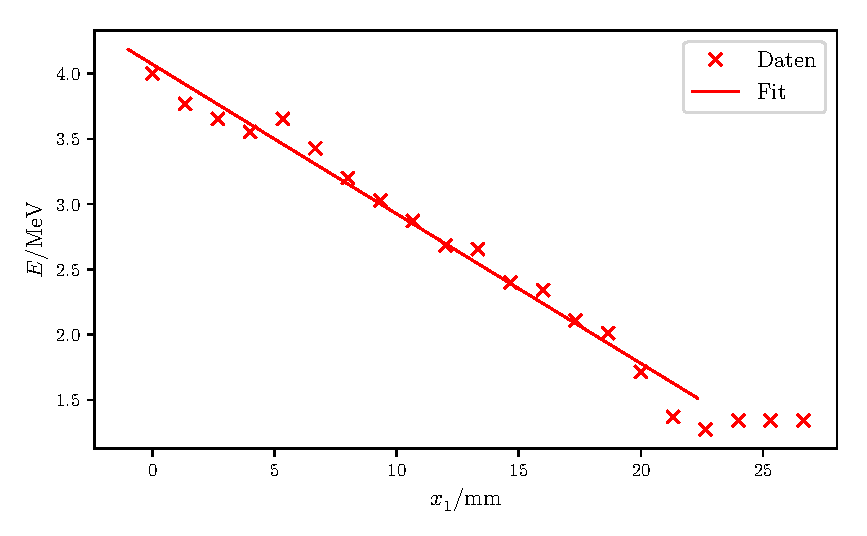
\includegraphics[width=15cm, height=9cm]{build/plotb.pdf}
    \caption{Hier ist die Länge gegen die jeweilige Energie aufgetragen.}
    \label{fig:energie1}
\end{figure}

\noindent Die Fitparameter der linearen Regression mit einer allgemeinen Gleichung \eqref{linReg} ergeben sich dadurch zu 
\begin{align*}
    m &= - \SI{0.1145(42)}{\mega\electronvolt\per\milli\per\meter} \\
    n &= \SI{4.070}{\mega\electronvolt} .
\end{align*}

\noindent Daraus lässt sich anhand der Steigung der Energieverlust der Strahlung bestimmen %wie genau?
\begin{equation*}
    - \left( \frac{dE}{dx} \right)_1 = - \SI{0.1145(45)}{\mega\electronvolt\per\milli\per\meter}.
\end{equation*}

\subsubsection{Zweiter Abstand}
Die Drücke, die Anzahl der Pulse und die Position des jeweiligen Maximums für den Abstand $d_2 = \SI{2}{\centi\meter}$ in Tab. \ref{tabb} zu sehen.
 
 \begin{table}\caption{Die angelegte Spannung des elektrischen Feldes innerhalb des Geiger-Müller-Zählrohrs, die Anzahl der jeweils gemessenen Impulse und der Strom innerhalb des Geiger-Müller-Zählrohrs.}
\label{tabb}
\centering
\sisetup{round-mode = places, round-precision=2, round-integer-to-decimal=true}
\begin{tabular}{c c S[]} 
\toprule
{$U / \si{\volt}$} & {$\frac{N}{\SI{130}{\second}}$} & {$I / \si{\ampere}$}\\
\midrule
320 & 11298 & 0.1\\
400 & 11820 & 0.2\\
480 & 12135 & 0.3\\
540 & 12301 & 0.35\\
560 & 12068 & 0.4\\
600 & 12354 & 0.45\\
640 & 12403 & 0.5\\
660 & 12507 & 0.55\\
680 & 12659 & 0.6\\
\bottomrule
\end{tabular}\end{table}

%Zählrate als Funktion der effektiven Länge für den ersten Abstand
\noindent Die mit Gleichung \eqref{eqn:x} ermittelten Abstände, die Anzahl der Pulse (Zählrate) und die mit Gleichung \eqref{eqn:energie} ermittelten Energien befinden sich in Tab. \ref{tab2}. 

 \begin{table}\caption{Das Verhältnis des magnetischen Feldes durch die Beschleunigungsspannung aufgetragen gegen die Höhe.}
\label{tab2}
\centering
\sisetup{round-mode = places, round-precision=2, round-integer-to-decimal=true}
\begin{tabular}{S[]S[]S[]} 
\toprule
{$B_1 / \si{\henry}$} & {$B_2 / \si{\henry}$} & {$\frac{D}{(L^2 + D^2)} / \si{\per\meter}$}\\
\midrule
0.0 & 0.0 & 0.0\\
3.5649278338607584e-07 & 3.862005153349155e-07 & 0.29289724188430566\\
8.912319584651897e-07 & 8.912319584651897e-07 & 0.5827222842713544\\
1.4259711335443034e-06 & 1.396263401595464e-06 & 0.8665094112549946\\
1.9250610302848096e-06 & 1.8418793808280586e-06 & 1.1414982164090373\\
2.3885016486867084e-06 & 2.3172030920094934e-06 & 1.4052180429996723\\
2.923240823765822e-06 & 2.822234535139767e-06 & 1.6555530006898145\\
3.4223307205063282e-06 & 3.3272659782700412e-06 & 1.8907846756403912\\
\bottomrule
\end{tabular}\end{table}

\noindent Die Zählrate ist in Abb. \ref{zaehlrate2} gegen die mit Gleichung \eqref{eqn:x} bestimmte effektive Länge aufgetragen.

\begin{figure}
    \centering
    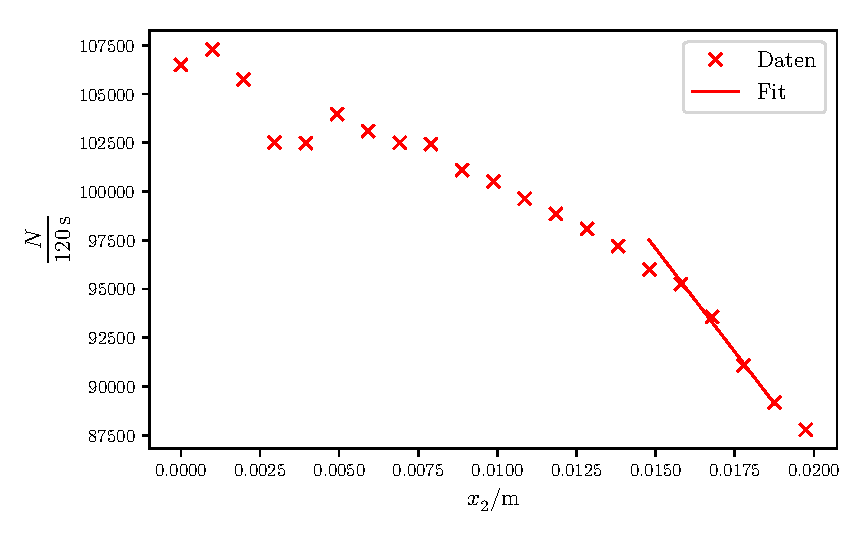
\includegraphics[width=15cm, height=9cm]{build/plotc.pdf}
    \caption{Anzahl der Hits pro zwei Minuten Messzeit ist hier gegen den Abstand aufgetragen. Dabei wurde dieses Ergebnis durch die Abhängigkeit vom jeweiligen Druck ermittelt.}
    \label{zaehlrate2}
\end{figure}

\noindent Die Fitparameter der linearen Regression ergeben sich dadurch mit einer allgemeinen Gleichung \eqref{linReg} zu 
\begin{align*}
    m &= -\num{839.54(3085)}\, \frac{\text{N}}{\SI{120}{\second} \, \si{\milli\meter}} \\
    n &= \num{108514.077} \, \frac{\text{N}}{\SI{120}{\second}} .
\end{align*}


\noindent Mit dem Umformen dieser linearen Gleichung ergibt sich bei $y = \frac{1}{2} max$ die mittlere Reichweite der $\alpha$-Teilchen zu dem Wert %wie genau?
\begin{equation*}
    R_\text{m,2} = \SI{65.8(24)}{\milli\meter}
\end{equation*}
bestimmen.

\noindent Das entspricht nach Formel \eqref{eqn:Rm} einer Energie von %wie genau?
\begin{equation*}
    E_2 = \SI{7.67(19)}{\mega\electronvolt}.
\end{equation*}

%Energie als Funktion der effektiven Länge für den ersten Abstand
\noindent Die Energie aus Tab. \ref{tab2} ist in Abb. \ref{fig:energie2} gegen die effektive Länge aufgetragen.
\begin{figure}
    \centering
    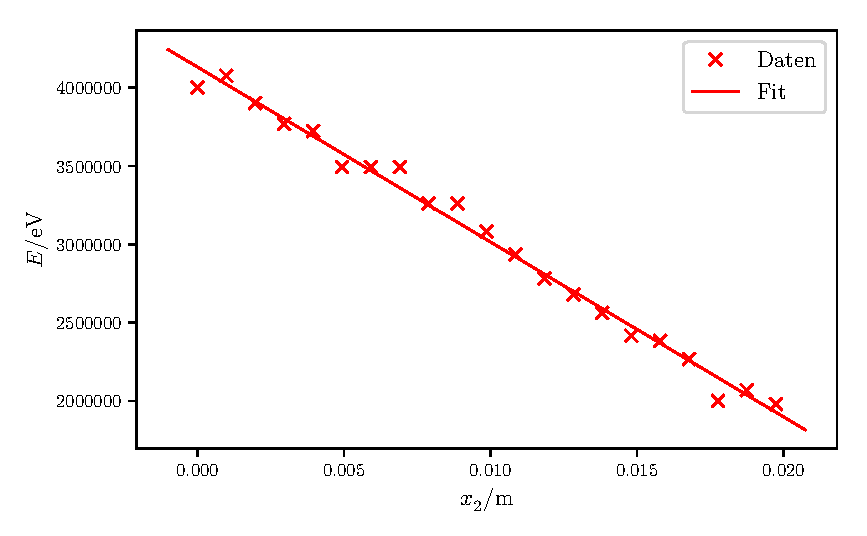
\includegraphics[width=15cm, height=9cm]{build/plotd.pdf}
    \caption{Hier ist die Länge gegen die jeweilige Energie aufgetragen.}
    \label{fig:energie2}
\end{figure}

\noindent Die Fitparameter der linearen Regression ergeben sich dadurch zu 
\begin{align*}
    m &= -\SI{0.1117(26)}{\mega\electronvolt\per\milli\per\meter} \\
    n &= \SI{4.1327}{\mega\electronvolt} .
\end{align*}

\noindent Daraus lässt sich anhand der Steigung der Energieverlust der Strahlung bestimmen %wie genau?
\begin{equation*}
    - \left( \frac{dE}{dx} \right)_2 = - \SI{0.1117(26)}{\mega\electronvolt\per\milli\per\meter}.
\end{equation*}

\subsection{Untersuchung der Statistik des radioaktiven Zerfalls}

Die Anzahl der Pulse, die jeweils in $\SI{10}{\second}$ gemessen wurde, sind in Tab. \ref{tabc} eingetragen.

\begin{table}\caption{Der Anodenstrom und der Kathodenstrom bei einer Beschleunigungsspannung von $U_\text{B} = \SI{25}{\kilo\volt}$ und einer Kathodenspannung $U_\text{K,1} = \SI{500}{\volt}$ und einer Kathodenspannung $U_\text{K,2} = \SI{300}{\volt}$ bei einem Blendenradius von $r_\text{B} = \SI{5}{\milli\meter}$.}
\label{tabc}
\centering
\sisetup{round-mode = places, round-precision=2, round-integer-to-decimal=true}
\begin{tabular}{S[]S[]S[]} 
\toprule
{$I_\text{K} / \si{\milli\ampere}$} & {$I_\text{K,1} / \si{\nano\ampere}$} & {$I_\text{K,2} / \si{\nano\ampere}$}\\
\midrule
1.0 & 2.6 & 2.4\\
0.95 & 2.5 & 2.4\\
0.9 & 2.4 & 2.2\\
0.85 & 2.3 & 2.1\\
0.8 & 2.2 & 2.0\\
0.75 & 2.1 & 1.9\\
0.7 & 1.9 & 1.8\\
0.65 & 1.8 & 1.6\\
0.6 & 1.6 & 1.5\\
0.55 & 1.5 & 1.4\\
0.5 & 1.4 & 1.3\\
0.45 & 1.2 & 1.2\\
0.4 & 1.1 & 1.0\\
0.35 & 0.9 & 0.9\\
0.3 & 0.8 & 0.8\\
0.25 & 0.6 & 0.6\\
0.2 & 0.5 & 0.5\\
0.15 & 0.4 & 0.4\\
0.1 & 0.1 & 0.2\\
0.05 & 0.1 & 0.1\\
\bottomrule
\end{tabular}\end{table}

%Zerfallsraten in Histogramm
\noindent Die Zerfallsraten sind in Abb. \ref{fig:histogramm} in einem Histogramm aufgetragen. Außerdem ist eine Gauß- und eine Poissonverteilung nach Gleichung \eqref{eqn:gauss} und \eqref{eqn:poisson} aufgetragen. Bei der Erzeugung der beiden Verteilungen wurde ein Seed von 42 benutzt, um die Auswertung deterministisch zu machen. 
\begin{figure}
    \centering
    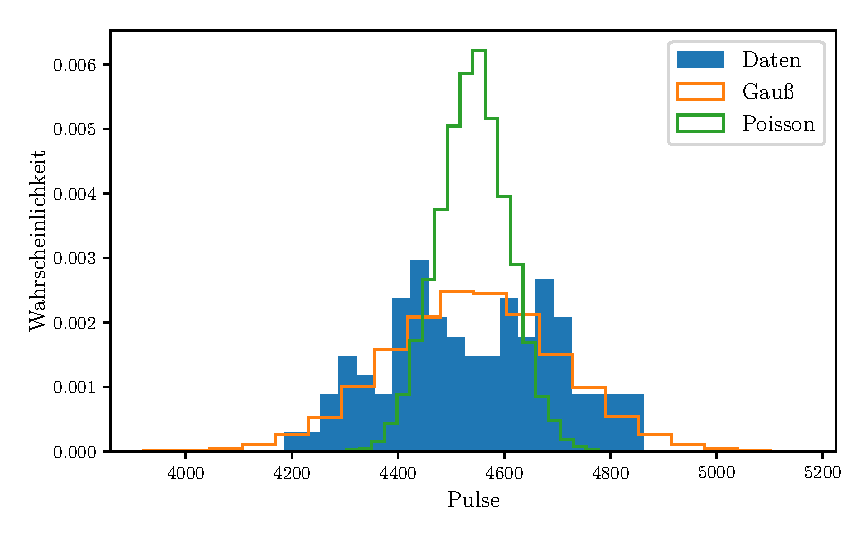
\includegraphics[width=15cm, height=9cm]{build/plote.pdf}
    \caption{Hier sind eine Gaussverteilung, eine Poissonverteilung und die tatsächlichen Messwerte gegeneinander aufgetragen.}
    \label{fig:histogramm}
\end{figure}

%Mittelwert und Varianz
\noindent Aus den gemessenen Zählraten lassen sich der  Mittelwert $\mu$ und die Varianz $\sigma^2$ bestimmen: %Gleichungen erwähnen, Varianz ergänzen?
\begin{align*}
    \mu &= \num{4541.6} \\
    \sigma^2 &= \num{25065.36}.
\end{align*}
